\begin{frame}{Energ\'ia de corte}
    \begin{columns}[t]
        \column{0.5\textwidth}
\begin{figure}[H]
    \centering
    \includegraphics[width=1.0\textwidth]{contenido/resultados/img_resultados/energia_corte_BFO.png}
    \caption{Energ\'ia de corte para el $BiFeO_{3}$}
\end{figure}
        \column{0.5\textwidth}
\begin{figure}[H]
    \centering
    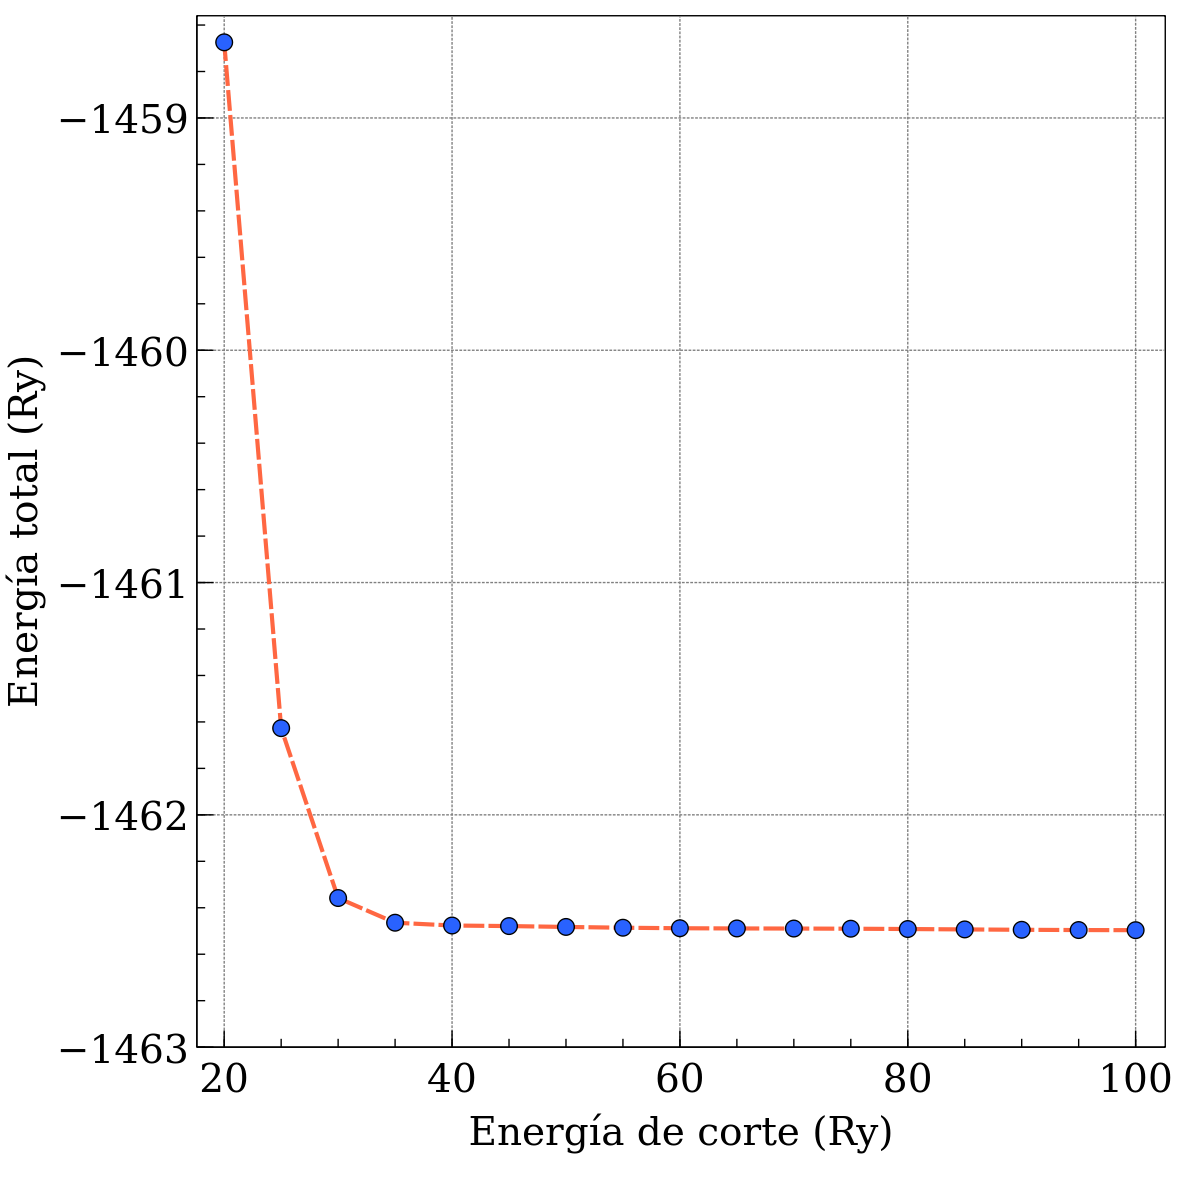
\includegraphics[width=1.0\textwidth]{contenido/resultados/img_resultados/energia_corte_YCO.png}
    \caption{Energ\'ia de corte para el $YCrO_{3}$}
\end{figure}
    \end{columns}
\end{frame}


\begin{frame}{Dimensi\'on de la grilla de puntos K}
        \begin{columns}[t]
            \column{0.5\textwidth}
\begin{figure}[H]
    \centering
    \includegraphics[width=1.0\textwidth]{contenido/resultados/img_resultados/energia_kp_BFO.png}
    \caption{Dimensi\'on de la grilla de puntos K para el $BiFeO_{3}$.}
\end{figure}
            \column{0.5\textwidth}
\begin{figure}[H]
    \centering
    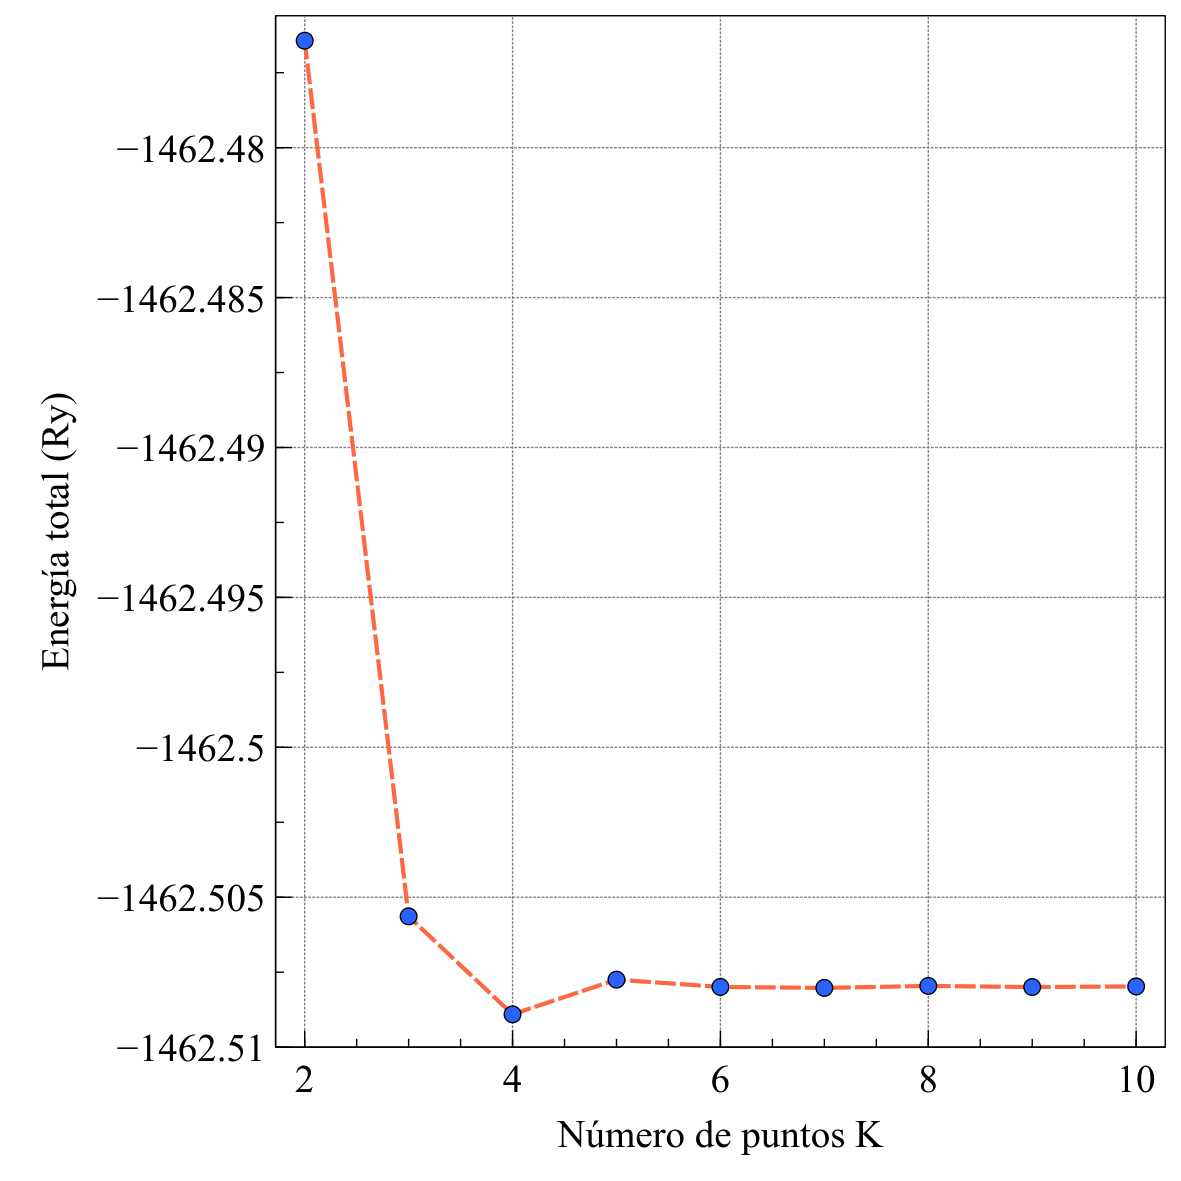
\includegraphics[width=1.0\textwidth]{contenido/resultados/img_resultados/energia_kp_YCO.png}
    \caption{Dimensi\'on de la grilla de puntos K para el $YCrO_{3}$.}
\end{figure}
        \end{columns}
\end{frame}